\documentclass[12pt,letterpaper]{article}
\usepackage[utf8]{inputenc}
\usepackage[spanish]{babel}
\usepackage{graphicx}
\usepackage[left=2cm,right=2cm,top=2cm,bottom=2cm]{geometry}
\usepackage{graphicx} % figuras
% \usepackage{subfigure} % subfiguras
\usepackage{float} % para usar [H]
\usepackage{amsmath}
%\usepackage{txfonts}
\usepackage{stackrel} 
\usepackage{multirow}
\usepackage{enumerate} % enumerados
\renewcommand{\labelitemi}{$-$}
\renewcommand{\labelitemii}{$\cdot$}
% \author{}
% \title{Caratula}
\begin{document}

% Fancy Header and Footer
% \usepackage{fancyhdr}
% \pagestyle{fancy}
% \cfoot{}
% \rfoot{\thepage}
%

% \usepackage[hidelinks]{hyperref} % CREA HYPERVINCULOS EN INDICE

% \author{}
\title{Caratula}

\begin{titlepage}
\begin{center}
\large{UNERSIDAD PRIVADA DE TACNA}\\
\vspace*{-0.025in}
\begin{figure}[htb]
\begin{center}

\includegraphics[width=7cm]{./Imagenes/logo}
\end{center}
\end{figure}
\vspace*{0.15in}
INGENIERIA DE SISTEMAS  \\

\vspace*{0.3in}
\begin{large}
\textbf{TITULO:} \\
\end{large}

\vspace*{0.1in}
\begin{Large}
\textbf{Trabajo Final Unidad I} \\

\end{Large}

\vspace*{0.3in}
\begin{Large}
\textbf{CURSO:} \\
\end{Large}

\vspace*{0.1in}
\begin{large}
INTELIGENCIA DE NEGOCIOS\\
\end{large}

\vspace*{0.3in}
\begin{Large}
\textbf{DOCENTE(ING):} \\
\end{Large}

\vspace*{0.1in}
\begin{large}
 Patrick Cuadros Quiroga\\
\end{large}

\vspace*{0.4in}
\vspace*{0.1in}
\begin{large}
\textbf{INTEGRANTE:} \\
\begin{flushleft}
Zavala Venegas, Luis Angel	\hfill	(2010037899)\\
Condori Quiso, Jesus		\hfill	(2008032440)\\
Condori Tito, Hernan		\hfill	(2009034553)

\centering  %CENTRA UN TEXTO
\vspace*{0.9in}
\begin{large}
Tacna\\ 29-10-2018
\end{large}


\end{flushleft}
\end{large}
\end{center}

\end{titlepage}


\tableofcontents % INDICE
\thispagestyle{empty} % INDICE SIN NUMERO
\newpage
\setcounter{page}{1} % REINICIAR CONTADOR DE PAGINAS DESPUES DEL INDICE


\section{Introdución} 
\vspace{12mm} %5mm vertical space


Los indicadores de desempeño son parámetros de medición de la actividad bibliotecaria. Su aplicación permite evaluar el rendimiento de la biblioteca y, por consiguiente, identificar sus logros y limitaciones en la prestación del servicio bibliotecario. Asimismo, su manejo proporciona información para la toma de decisiones y la asignación del presupuesto.
Los indicadores aquí señalados no son considerados como estándares que hay que cumplir, sino que actúan como un estímulo de mejora continua en la biblioteca y como un modo de subrayar las mejores prácticas. Su continuo manejo nos ayuda a priorizar los servicios bibliotecarios.
Podemos llevar a cabo la evaluación de la gestión bibliotecaria mediante la aplicación de indicadores y realizarla en diferentes períodos dentro de la misma biblioteca. También evaluamos valiéndonos de comparaciones entre bibliotecas, pero con extrema precaución, tomando en cuenta cualquier diferencia en la constitución de las mismas, o haciendo referencia a indicadores generales como la Norma ISO 11620 e interpretando los datos cuidadosamente. Debemos señalar que la norma no incluye indicadores para la evaluación del impacto de las bibliotecas en los usuarios o en la sociedad.



		


\section{Objetivos} 
\vspace{16mm} %5mm vertical space
\begin{center}
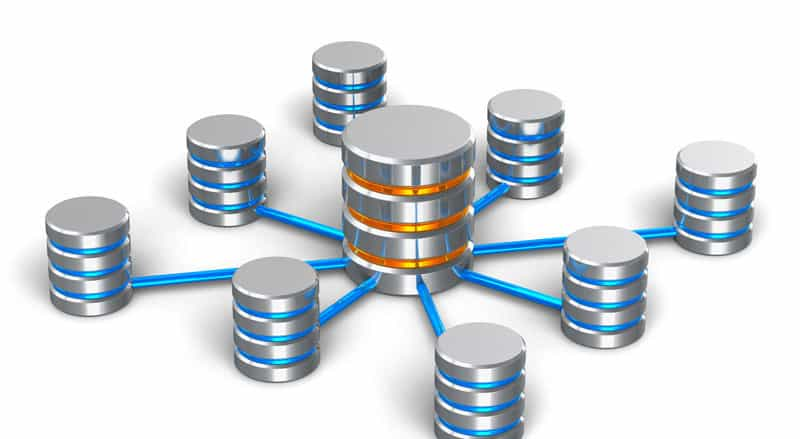
\includegraphics[width=17cm]{./Imagenes/001}
\end{center}	
\vspace{12mm} %5mm vertical space

\textbf{Objetivo:}\\

1. Servir de marco de referencia en materia de normatividad en gestión de bibliotecas universitarias. \\
2. Orientar la formulación de normas específicas para el funcionamiento de los procesos de gestión bibliotecaria en sus aspectos de desarrollo de colecciones, procesos técnicos, servicios e infraestructura. \\
3. Proteger y conservar los recursos de la biblioteca, asegurando que las operaciones se efectúen apropiadamente. \\
4. Controlar la efectividad y eficiencia de las actividades realizadas en las bibliotecas a fin de que estén enmarcadas dentro de los programas y presupuestos institucionales.





\section{Indicadores} 

\textbf{Lista de indicadores de desempeño para bibliotecas universitarias}\\

\vspace{16mm} %5mm vertical space
\begin{center}
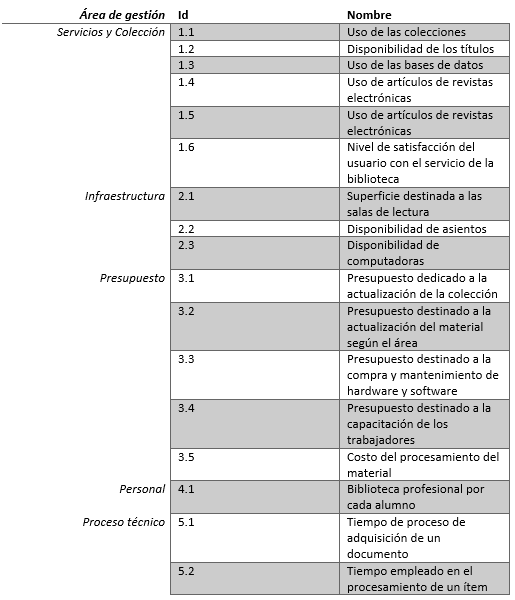
\includegraphics[width=17cm]{./Imagenes/002}
\end{center}	
\vspace{7mm} %3mm vertical space





\section{Modelo Dimensional} 

\textbf{Modelo Dimensional}
\vspace{5mm} %5mm vertical space

\vspace{5mm} %5mm vertical space
\begin{center}
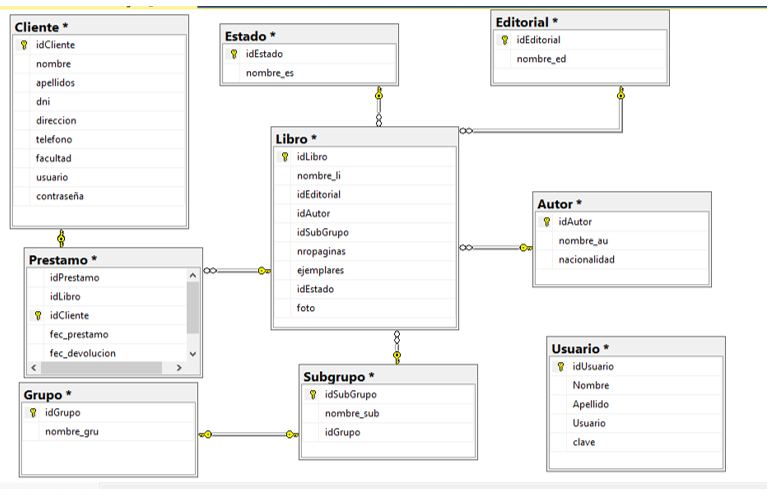
\includegraphics[width=19cm]{./Imagenes/003}
\end{center}	
\vspace{7mm} %3mm vertical space

\textbf{Base de Datos}\\

\vspace{3mm} %5mm vertical space
\begin{center}
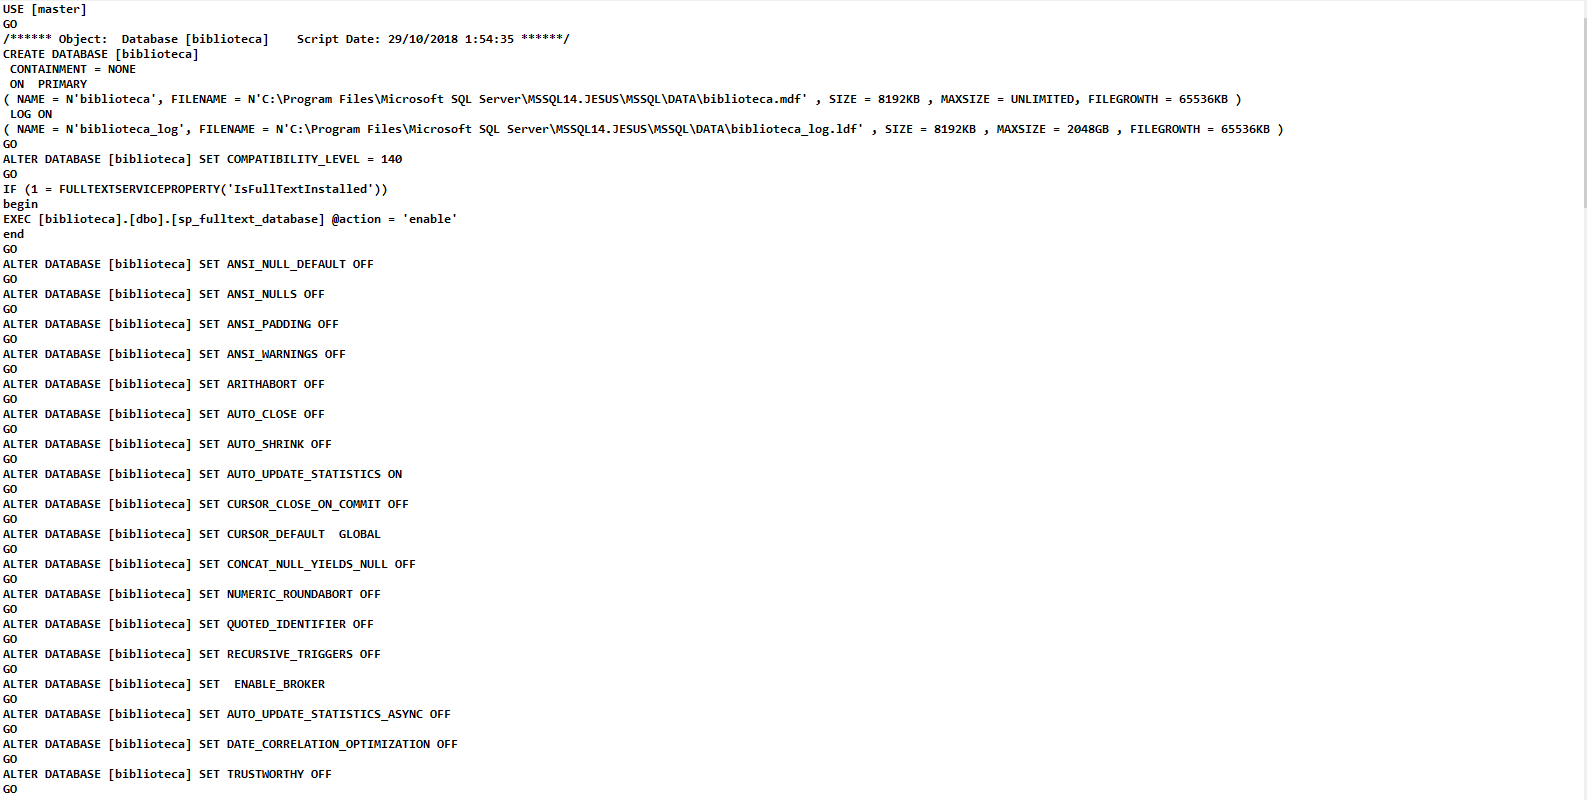
\includegraphics[width=19cm]{./Imagenes/005}
\end{center}	
\vspace{3mm} %3mm vertical space

\vspace{3mm} %5mm vertical space
\begin{center}
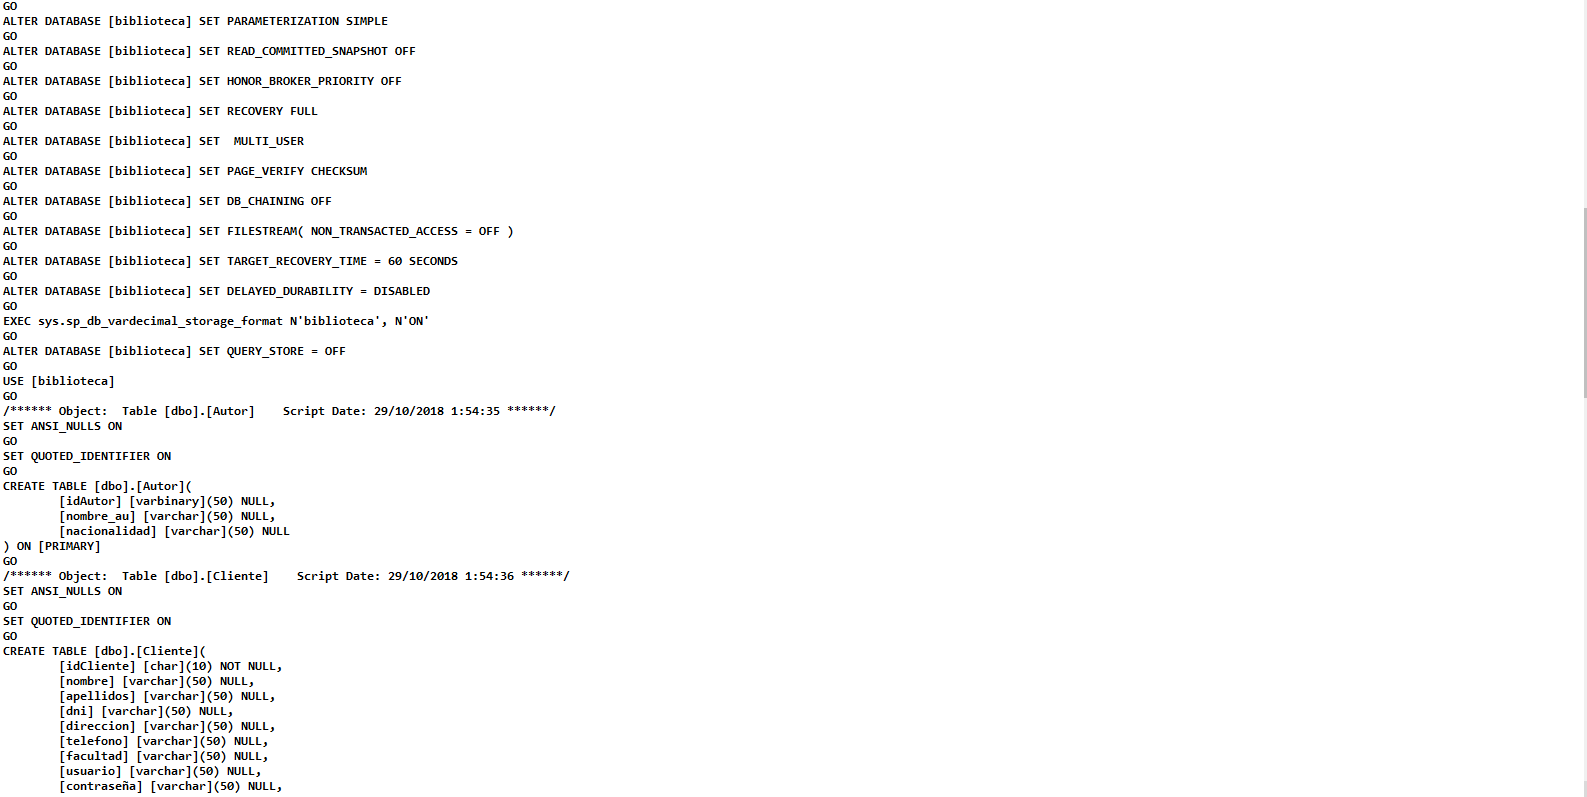
\includegraphics[width=19cm]{./Imagenes/006}
\end{center}	
\vspace{3mm} %3mm vertical space

\vspace{3mm} %5mm vertical space
\begin{center}
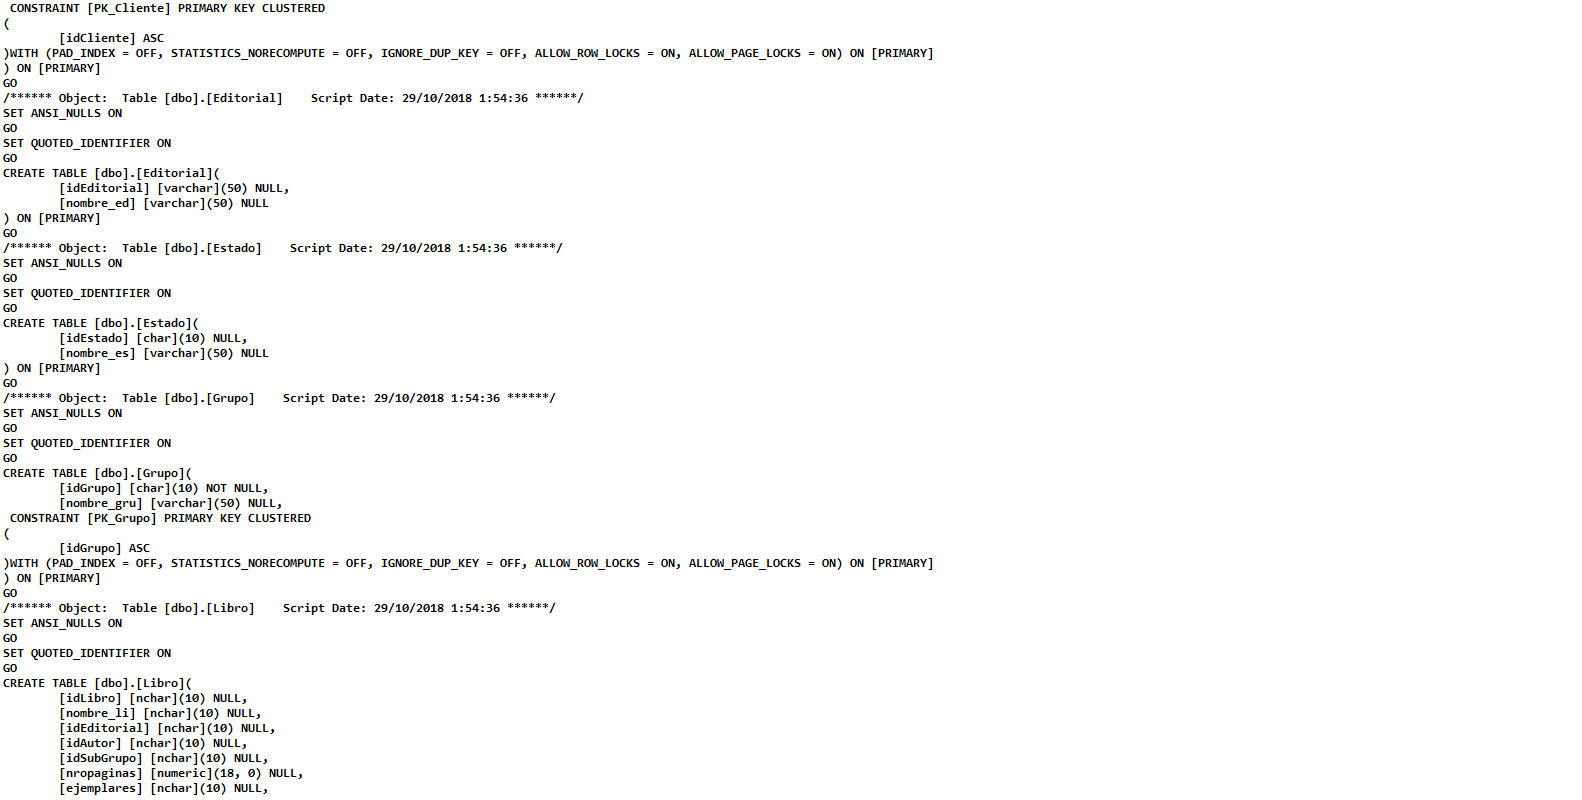
\includegraphics[width=19cm]{./Imagenes/007}
\end{center}	
\vspace{3mm} %3mm vertical space

\vspace{3mm} %5mm vertical space
\begin{center}
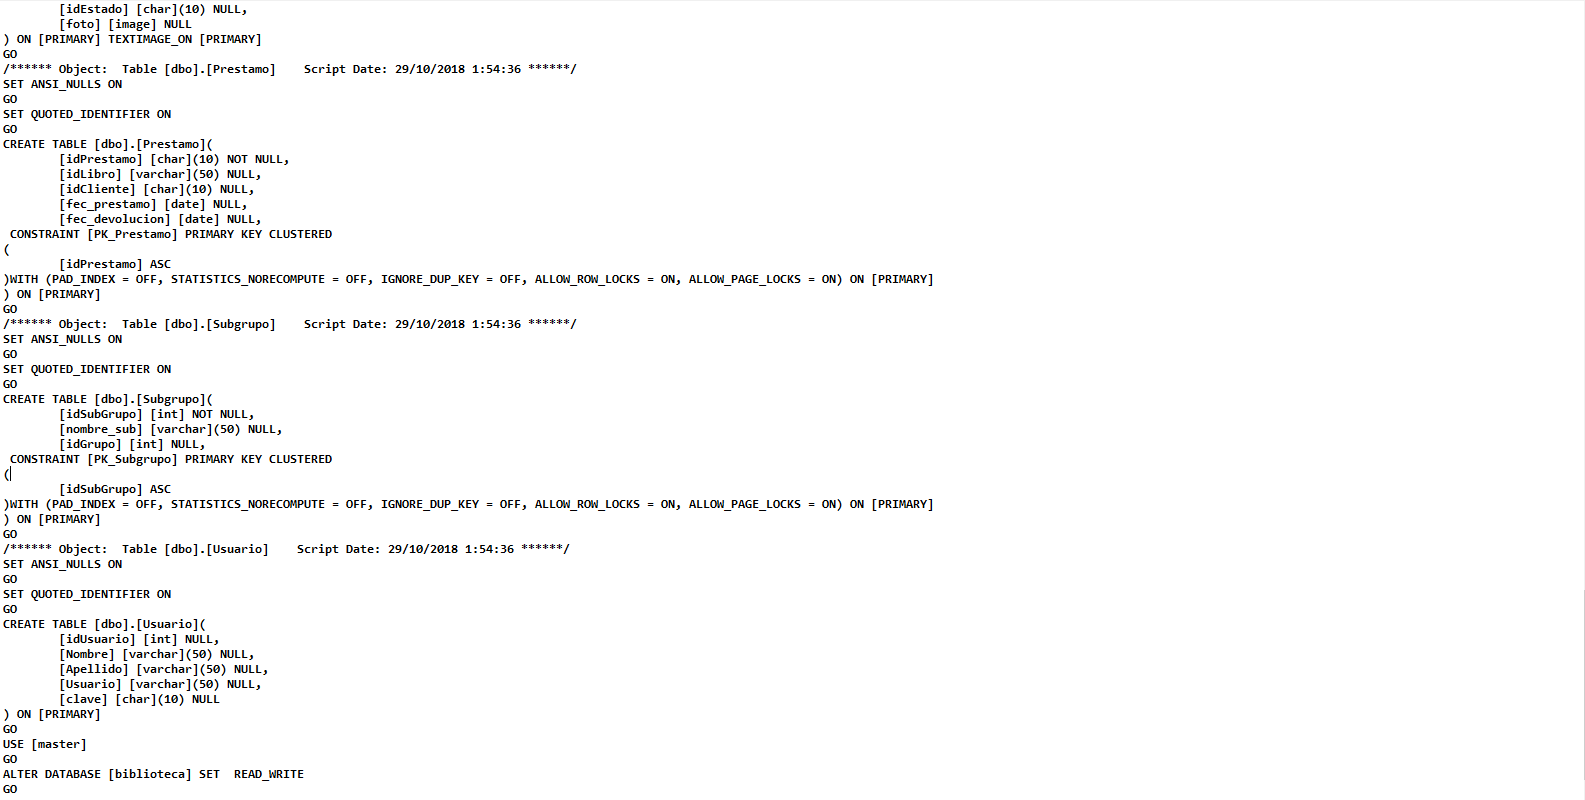
\includegraphics[width=19cm]{./Imagenes/008}
\end{center}	
\vspace{3mm} %3mm vertical space









\end{document}
